In order to allow further experimentation and expansion of the tool, we aimed to implement a model with a highly object oriented framework so that the different parts of the tool could be replaced by new ones smoothly. Therefore, for the writing of the script, Java programming was used for two reasons: First of all, Java is a popular programming language; and second, it opens up the possibility of using the tool with many other packages or even as a webservice for more sophisticated applications.
\subsection{Java Packages}
\emph{Description of the most important  packages and classes related to the implementation:}
\subsubsection*{IO}
\begin{enumerate}[-]
	\item The classes in this package deals with the input \& output files.
	\item The class \texttt{DictionaryReader.java} is in charge of reading a raw dictionary file \textit{(one entry per line).}
\end{enumerate}

\subsubsection*{Measures}
\begin{enumerate}[-]
	\item This package consists of all the classes related to the different similarity measures.
	\item The SimString algorithm works independently from the similarity measure that is choosen initially.
	\item A separate interface, named \texttt{Similarity} that chooses the similarity measure exists within the package.
	\item For the extension of the system to provide new similarity measures, this interface has to be implemented.
\end{enumerate}
Additionally, \texttt{Measures} package includes another class, named \texttt{"MeasureFactory"}. This class is in charge of constructing the similarities' of objects.

\begin{figure}[h!]
  \caption{Class Diagram with Respect to Similarity Classes}
  \centering
    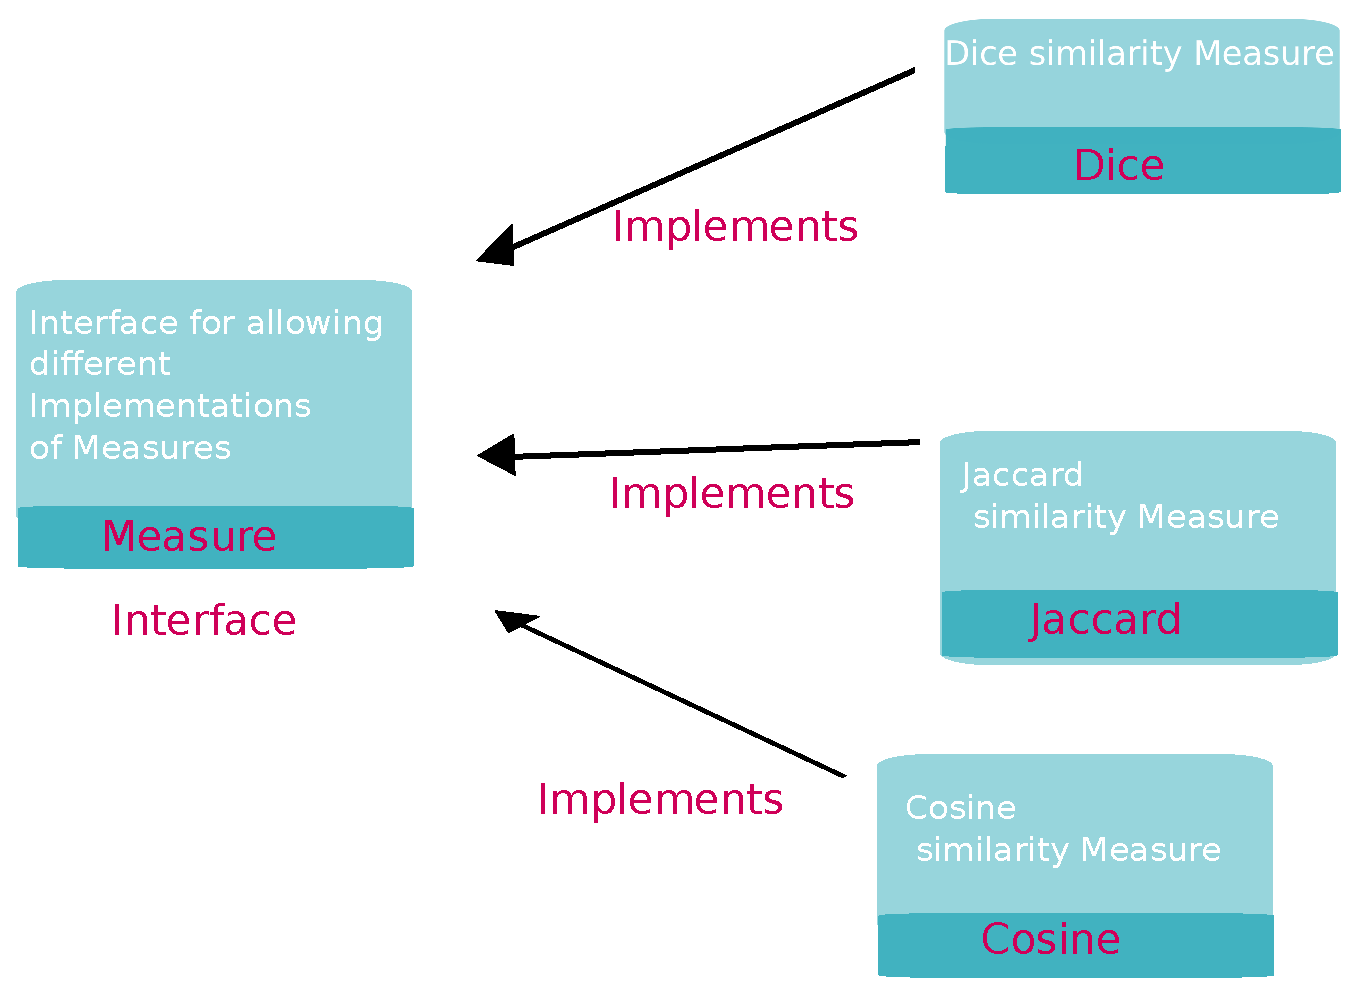
\includegraphics[scale=0.45]{graphics/similarities}
   \label{fig:similarityClasses}  
\end{figure}

\subsubsection*{Dictionary}
\begin{enumerate}[-]
	\item This package contains all the classes that are responsible for dictionaries.
	\item Besides the dictionary classes, this package also contains other classes related to the different implementations of dictionaries.
	\item One of the most important classes, named \texttt{LowLevelDictionaryImplementation}, is an interface that allows the system to implement different kinds of dictionaries.
	\item With this interface, a dictionary can be represented either as a hash table or as a suffix tree.
	\item Despite these dictionaries' different data structures, the \texttt{LowLevelDictionaryImplementation} interface makes them transparent to the SimString algorithm.
	%\item \textbf{DAVID: QUESTION: what about MemoryMapped Hash Table Dict.?}\textit{ Do we base the dictionary types only according to suffixTree / HashTable data types? Or did you forget to write about this?}
\end{enumerate}

\subsubsection*{SimString}
\begin{enumerate}[-]
	\item This package consists of the class \texttt{SimString}, which is responsible for retrieving all the similar Named Entities from the dictionaries. 
	\item With this class, for each dictionary, a similarity configuration and a query can search the dictionary and retrieve all the similar Named Entities according to its parameter values.
\end{enumerate}

\subsubsection*{Util}
\begin{enumerate}[-]
	\item This package consists of several classes with different responsibilities.
	\item The \texttt{N-gram} class is in charge of handling specific n-gram functionalities, such as splitting words into n-grams.
\end{enumerate}

\subsubsection*{Examples}
\begin{enumerate}[-]
	\item This package contains classes \textit{--each one of which is an example--} for the potential users.
\end{enumerate}

\subsubsection*{Test}
\begin{enumerate}[-]
	\item This package contains classes that allow developers to asses the time performance of the tool.
	\item For evaluation purposes, it makes comparisons of the different implementation models.
\end{enumerate}

\subsection{Dictionary Implementations}

As mentioned in the previous sections, as an addition to the \texttt{SimString} algorithm, we introduced three different models to implement the underlying data structure that represents the n-gram-inverted index. For the representation of this, we used two different data structure types:
\begin{enumerate}[i.]
	\item \texttt{Mapped Data Structure:} \textit{In this data structure type, data structures are saved in the hard disk, and small chunks of the data structures are loaded into memory on an on-demand / as-needed base.}
	\item \texttt{Not-Mapped Data Structure:} \textit{As it is the case with the traditional data structures, in this data structure type, the data structures are kept entirely on memory while the program is running.}
\end{enumerate}

The memory mapped data structures are ideally used for cases when the number of data that is being stored is very high, and thus having the whole data structure in memory at once is not always feasible. However, the memory mapped data structures come with a cost--that is--\texttt{Memory}.

Because the memory mapped data structure implementations aim to be as fast as traditional data structures; they have to be stored in memory in such a way that they can be retrieved quickly. The only way that enables this
is achieved by having a fixed number of bits used per data field in the mapped data structure. In other words, this means that no matter what the size of the data is, a slot in this structure will always have a fixed-size. However, having this specific structure with a fixed-size slot results in using extra memory.

\begin{figure}[h!]
  \caption{The Dictionary Implementations}
  \centering
    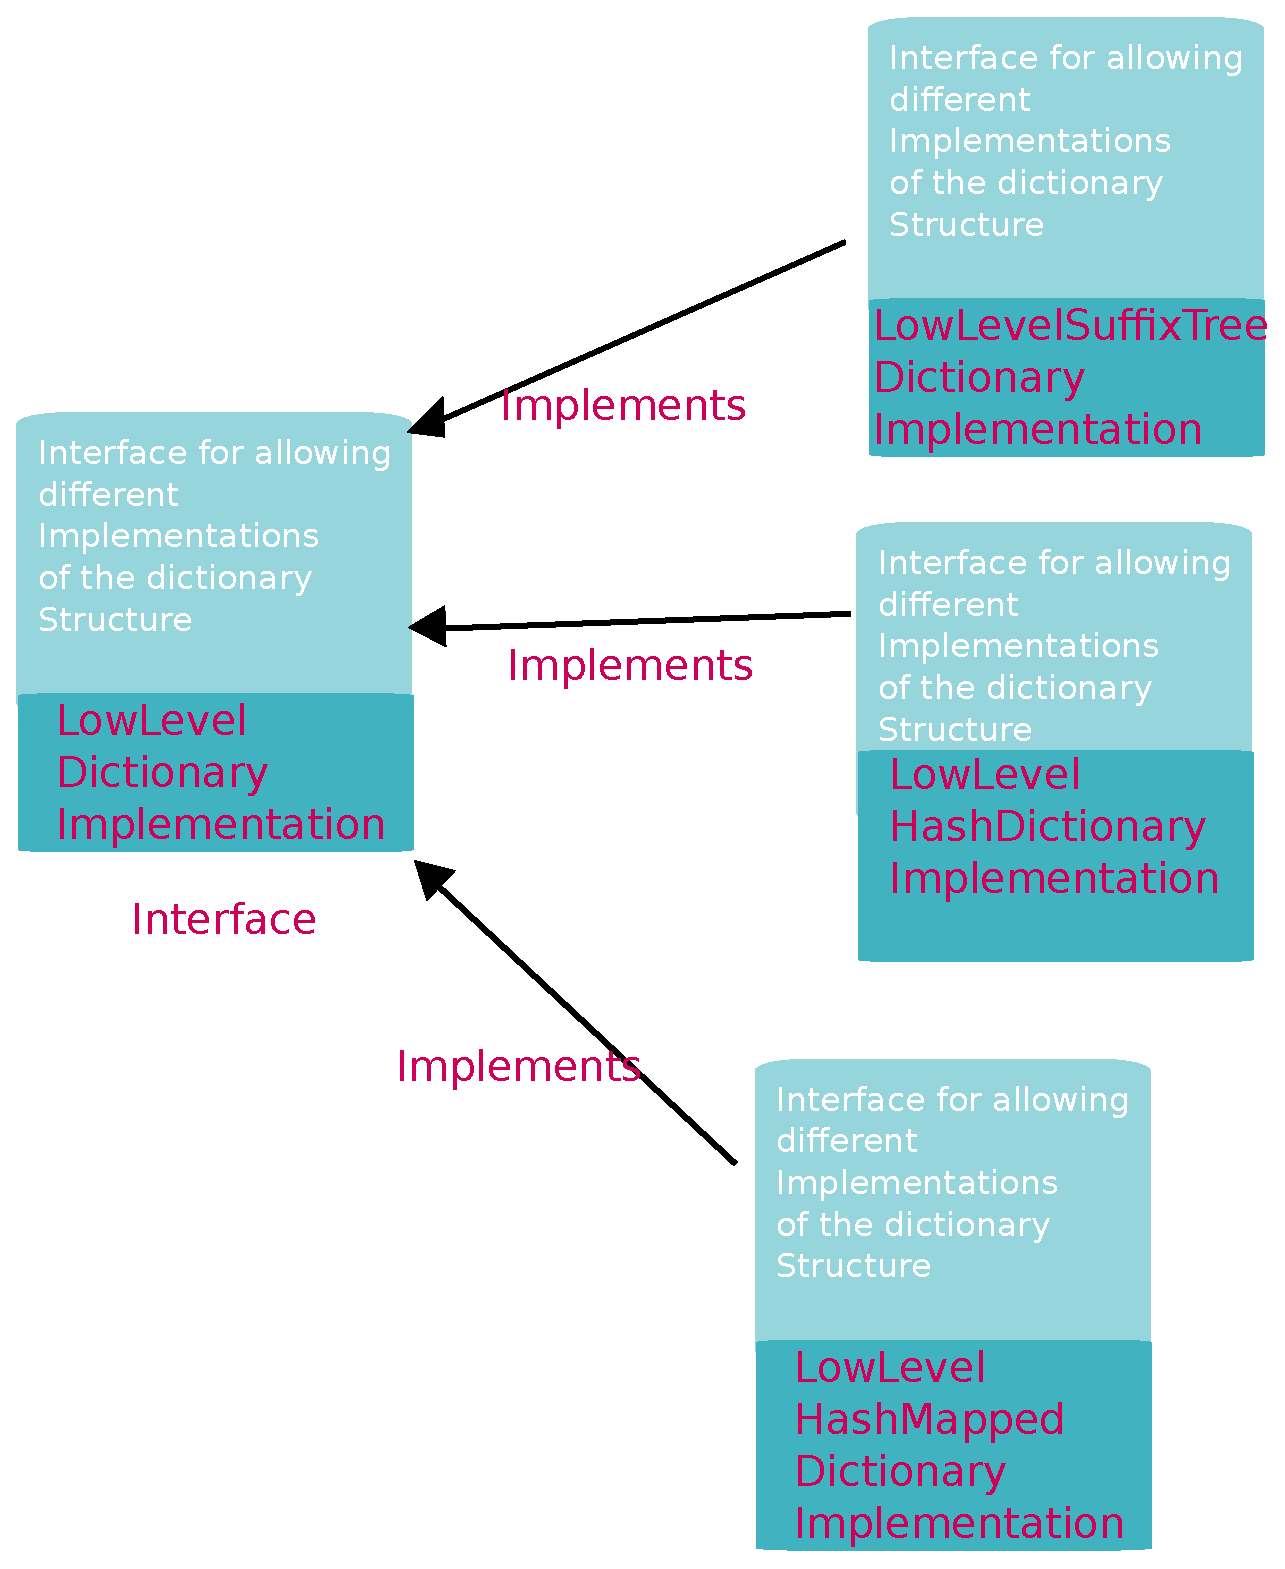
\includegraphics[scale=0.45]{graphics/dictionaryImplementations}
   \label{fig:dictionaryClasses}  
\end{figure}

\subsubsection{SuffixTree}  
This is an implementation of the inverted index of n-grams, using suffix trees. The keys in this model are made from the strings of the shape\texttt{ `ngram-sizeOfString.'} The values are priority queues with the IDs of dictionary entries, in which the size is \texttt{sizeOfString}, consisting of the given \texttt{ngram}.

\subsubsection{Naive-HashTable}
This is an implementation of the inverted index of n-grams that uses Java HashMaps. The keys in this model are made from the strings of the shape\texttt{ `ngram-sizeOfString.'} The values are priority queues with the IDs of dictionary entries, in which the size is \texttt{sizeOfString} and contains the given \texttt{ngram}.
  
\subsubsection{MemoryMapped Hashtable}
This is an implementation of the inverted index of n-grams that uses memory mapped hash tables. It enables the generated dictionary to be saved in a file, and to be loaded for later use.

\begin{figure}[h!]
  \caption{Comparison between Mapped \& Not-Mapped Data Structures}
  \centering
    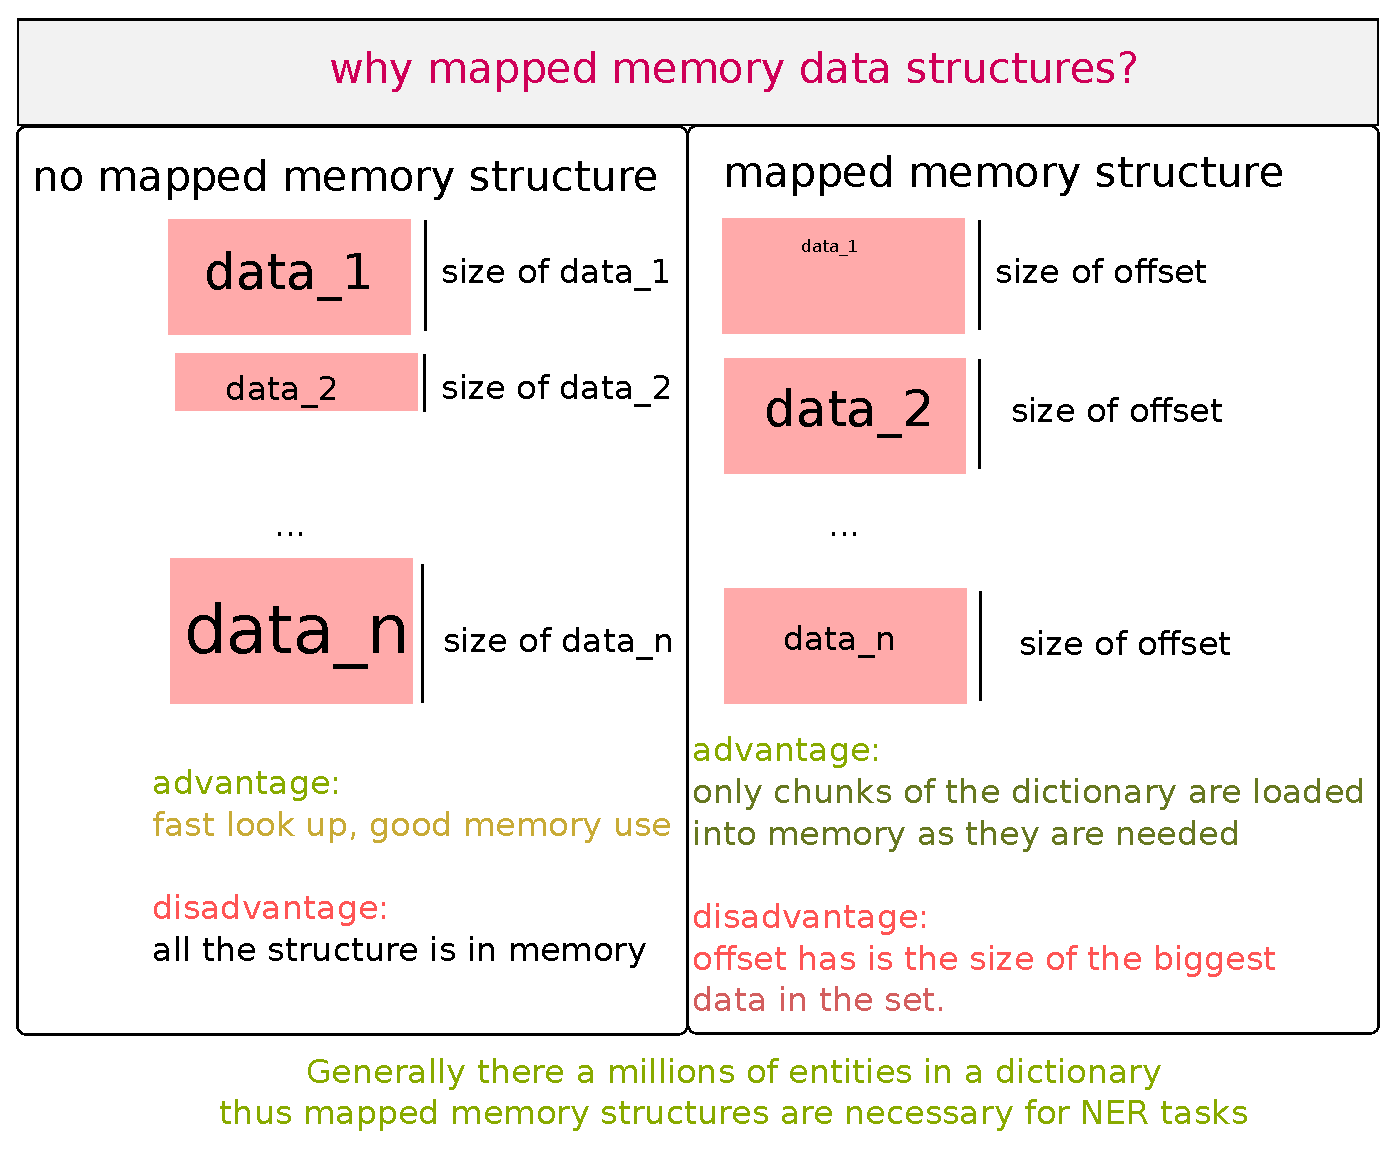
\includegraphics[scale=0.5]{graphics/memoryMappedVsNonMemoryMapped}
   \label{fig:mappedDataStructures}  
\end{figure}


  
